%E_Exp_3

This experiment mirrors Experiment 2, but focussing on instructions that did not use a number. We manipulated vagueness and the selection task (comparison and matching). In order to implement the experiment without mentioning numbers in the instructions, we changed the sequence of each trial to include a `target' (i.e., a dot array of a particular cardinality) before the array, so that we could then refer to the target's cardinality in the instruction using expressions like \emph{the same number of dots as the target}; \emph{fewer dots than the target}. An example of this sequence is given in Figure \ref{Experiment3examplestimulus}. This presentation of a target before the main body of the trial shares some features with \citeauthor[Experiment 2]{Izard20081221}, although in that experiment participants were told the cardinality of the target (called an \emph{inducer} in that paper) whereas in our experiment we did not tell participants the cardinality of the prime array. An item was thus a combination of a target dot array, an instruction that did not contain a number, and a set of dot arrays taking their cardinalities from the same triples used in Experiments 1 and 2. Table \ref{instructionsE-exp-3} spells out how the instructions were constrained not to mention a numeral and gives examples of targets.

\begin{figure}[htbp]
\centering
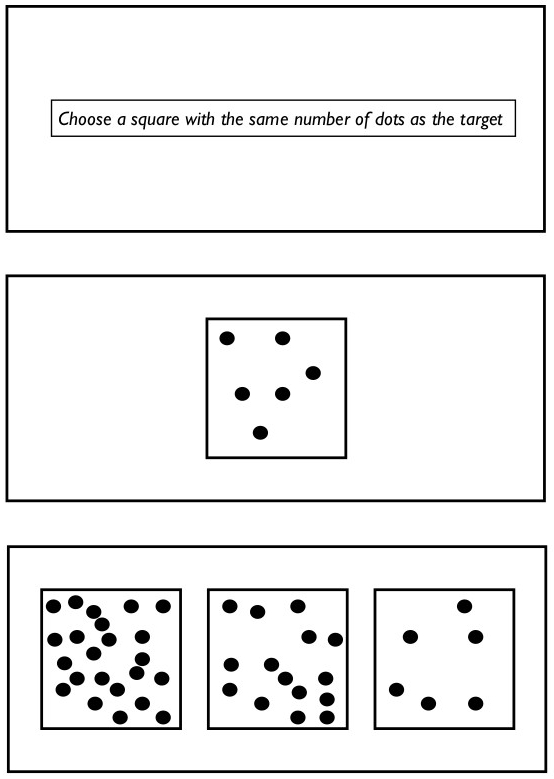
\includegraphics[width=.5\textwidth]{figures/Ee3-flow.jpg}
\caption{Experiment 3 example stimulus, showing the sequence of presentation, with the instruction screen at the top, followed by the presentation of the "target" array, followed by the stimulus that participants responded to.}
\label{Experiment3examplestimulus}
\end{figure}

\begin{table}
\centering
\caption{Experiment 3 instructions for the smallest array, arranged by condition. The instructions given in the table started with ``Choose a square with \ldots"}
\label{instructionsE-exp-3}
\resizebox{\textwidth}{!}{\begin{tabular}{ccccl}
\hline\noalign{\smallskip}
Item & Target & Selection & Vagueness & Instruction \\ 
\noalign{\smallskip}\hline\noalign{\smallskip}
06:15:24 &   6 & Matching 	& Crisp 	& the same number of dots as the target 	    \\ 
06:15:24 &  10 & Matching	& Vague		& about the same number of dots as the target	\\
06:15:24 &  20 & Comparison & Crisp 	& fewer dots than the target             	    \\ 
06:15:24 &  20 & Comparison	& Vague		& far fewer dots than the target				\\
\noalign{\smallskip}\hline
\end{tabular}}
\end{table}

\subsection{Hypotheses (Experiment 3)}

For Experiment 3, we hypothesised:

\begin{description}
	\item [Hypothesis 1 (Crisp/Vague RT)] Vague instructions are easier for the reader than crisp ones.
	\item [Hypothesis 2 (Comparison/Matching RT)] Comparison is easier for the reader than matching.
	\item [Hypothesis 3 (Interaction)] The effect of vagueness differs depending on whether the selection task mandated by the instructions is matching or comparison.
\end{description}

\subsection{Results (Experiment 3)}

40 volunteers participated. Response times from all trials were trimmed at 2.5 standard deviations for each subject, leading to the loss of 211 trials (2.8\% of the trials). The distribution of remaining response times was skewed with many long responses. These remaining response times were log-transformed which reduced this skew so that their distribution more closely approximated a normal distribution. Condition means for response times are plotted in Figure \ref{resultsE-exp-3}.

\begin{figure}[htbp]
\centering
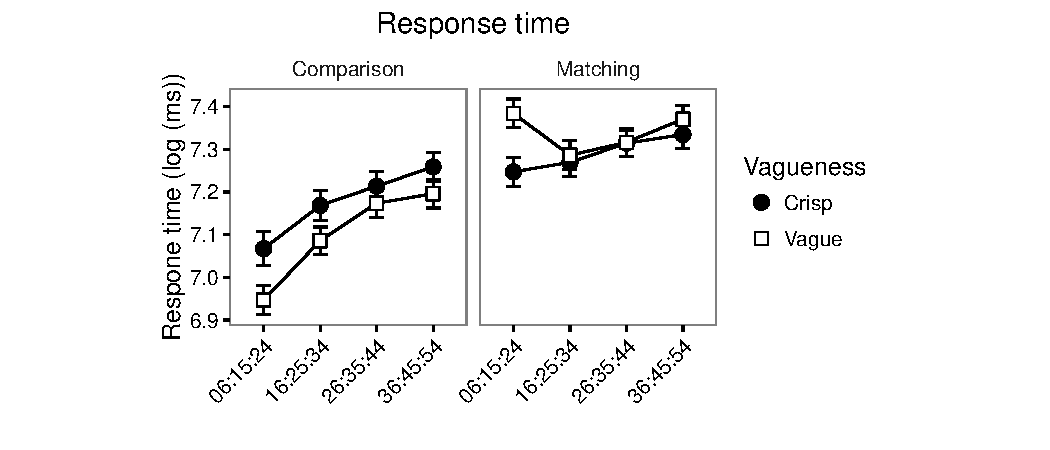
\includegraphics[width=\textwidth]{figures/Ee3-rtplot-1.pdf}
\caption{Mean response times by condition for Experiment 3 where all instructions were verbal}
\label{resultsE-exp-3}
\end{figure}

A linear mixed model was constructed for the logged response times, with sum-coded vagueness, selection task, and their interaction, and item as fixed effects, and per-participant intercepts and slopes for sum-coded vagueness, selection task, and their interaction, and item for random effects.

\begin{description}
	\item [Test of Hypothesis 1 (Crisp/Vague RT)] Vague instructions resulted in faster responses than crisp instructions on average. However this difference was not significant in the full model ($\beta=-0.015$, $se=0.0097$, $t=-1.58$, $p=0.119$). Using Levy's method \citep{Levy:MainEffectsInteractions} to test for main effects in the presence of higher-order interactions, by doing model comparison between a null model that included all interaction terms involving Vagueness but leaving out a term for the main effect of Vagueness, against a full model that differed only by including Vagueness as a main effect, showed that the full model was no better than the reduced model ($df=1$, $p=0.118$), consituting more evidence that Vagueness did not exert a significant main effect on response times. 
	\item [Test of Hypothesis 2 (Comparison/Matching RT)] Comparison instructions resulted in significantly faster responses than matching instructions ($\beta=0.176$, $se=0.0168$, $t=10.51$, $p<0.001$).
	\item [Test of Hypothesis 3 (Interaction)] The interaction between Vagueness and Selection task was significant ($\beta=0.123$, $se=0.0166$, $t=7.42$, $p<0.001$), showing that Vagueness had a different influence on response times when the instructions mandated comparison versus when the instructions mandated matching. When separate analyses were carried out testing for the effect of vagueness in comparison-only and in matching-only conditions, vague instructions led to significantly \emph{faster} responses than crisp instructions in the comparison-only conditions ($\beta=-0.077$, $se=0.018$, $t=-4.31$, $p<0.001$); and in the matching-only conditions vague instructions led to significantly \emph{slower} responses than crisp instructions ($\beta=0.047$, $se=0.013$, $t=3.71$, $p<0.001$).
\end{description}

\subsection{Discussion (Experiment 3)}

The cost reduction account predicted that there should be a significant main effect of Vagueness such that responses would be faster for Vague intructions than for crisp instructions. We found that although there was a very small effect in that direction, the effect was not statistically significant. Models that differed only in the presence of Vagueness as a main effect were shown not to differ significantly in their explanatory value. 

However, the results also showed that vagueness did exert an influence on reaction times according to whether the task was comparison or matching: vagueness was beneficial for comparison and detrimental for matching (the same as Experiment 2) even when no numbers were allowed in the instructions. 
